
\documentclass[12pt,a4paper]{article}

% ---- Packages ----
\usepackage[margin=1in]{geometry}
\usepackage{amsmath,amssymb}
\usepackage{graphicx}
\usepackage{hyperref}
\usepackage{booktabs}
\usepackage{caption}
\usepackage{subcaption}
\usepackage{natbib}
\usepackage{float}
\usepackage{xcolor}

\title{\textbf{EcoEcon: Ecological Resilience Indicators for Systemic Risk---A Retrospective Analysis of the 2008 Financial Crisis with a 2020 Negative Control}}

\author{
    Abhinav Vaddi\\
    \texttt{github.com/Abhiv1028/EcoEcon}
}

\date{\today}

\begin{document}

\maketitle

\begin{abstract}
Can ecological collapse theory provide early warning indicators for financial crises?
We model the US economy as a biological ecosystem---sectors as species, supply chains
as mutualistic dependencies, and bankruptcy cascades as extinction events---and apply
three bodies of ecological theory to BEA Input-Output and FRED data: May's (1972)
stability theorem, Scheffer et al.'s (2009) critical slowing down, and network
robustness metrics. We construct an Economic Biodiversity Index (EBI), track network
spectral gap, and compute critical slowing down signals across two episodes: the 2008
Global Financial Crisis (endogenous fold bifurcation, signal expected) and the 2020
COVID shock (exogenous perturbation, no signal expected by theory). In a retrospective
analysis, two of five ecological signals behaved as theorized before 2008: spectral gap
declined monotonically 2002--2007 (Kendall $\tau = -0.87$) and housing starts variance
peaked approximately 18 months before crisis onset. Logistic regression trained on these
features achieves leave-one-out AUC = 1.000 ($p = 0.034$, permutation test) with zero
false positives in cross-validation. The 2020 negative control holds: models trained on
2008 assign near-zero crisis probability to 2015--2019, and four of five ecological
signals show no pre-crisis buildup before the exogenous COVID shock, consistent with
the theoretical prediction. Spectral gap produces zero false alarms across ten calm-period
years (2010--2019). This analysis is explicitly retrospective and limited to one positive
crisis episode; generalizability requires multi-crisis validation. We propose ecological
resilience indicators as a theoretically grounded and empirically promising direction for
systemic risk research.
\end{abstract}

% ============================================================
\section{Introduction}
% ============================================================

Financial crises remain notoriously difficult to predict. Standard early warning systems
rely on macroeconomic aggregates---credit growth, asset prices, current account
deficits---yet the 2008 Global Financial Crisis exposed the limitations of these
approaches: most official forecasts in 2007 projected continued growth
\citep{reinhart2009}.

Ecology faces a structurally analogous problem: detecting when a stable ecosystem is
approaching collapse. Over five decades, ecologists have developed a robust theoretical
framework for understanding stability and collapse in complex systems. \citet{may1972}
proved that complexity itself can be destabilizing---above a critical threshold of
diversity and connectance, large random systems become inherently unstable.
\citet{scheffer2009} demonstrated that many complex systems exhibit ``critical slowing
down'' before tipping points: rising variance and autocorrelation in key state variables
as the system loses resilience. \citet{acemoglu2015} showed that financial networks
exhibit phase transitions where diversification reduces individual risk up to a point,
beyond which it amplifies systemic fragility through contagion channels.
\citet{haldane2011} applied this ecological analogy directly to banking systems,
demonstrating that the same complexity-fragility tradeoff governs interbank contagion
networks.

This paper operationalizes the ecology-economy analogy by constructing ecological
metrics from economic data and testing whether they were elevated before the 2008
crisis. Critically, we also test a theoretically motivated \textit{negative control}:
the 2020 COVID shock was an exogenous perturbation rather than an endogenous approach
to a bifurcation, so ecological theory predicts that critical slowing down signals
should \textit{not} appear before 2020. This contrast---signal before an endogenous
crisis, no signal before an exogenous shock---provides stronger evidence than a single
positive episode alone.

We make no claim that these signals would have been detectable in real time or that
they generalize beyond this single positive episode. That question requires multi-crisis
validation outside the scope of this retrospective study.

% ============================================================
\section{Methods}
% ============================================================

\subsection{Variable Mapping}

Table~\ref{tab:mapping} presents the ecological-to-economic translation underlying our
metrics. We note one important theoretical correction relative to standard ecological
analogies: supplier-buyer relationships in IO networks are structurally closer to
\textit{mutualistic} interactions (+/+) than predator-prey interactions (+/$-$), since
both parties benefit from the transaction. This distinction matters because
\citet{allesina2012} showed that mutualistic networks destabilize more rapidly with
increasing diversity and connectance than predator-prey networks---placing economic IO
networks in a potentially more fragile stability regime than the predator-prey framing
would imply.

\begin{table}[H]
\centering
\caption{Ecological-to-economic variable mapping}
\label{tab:mapping}
\begin{tabular}{ll}
\toprule
\textbf{Ecological Concept} & \textbf{Economic Analog} \\
\midrule
Species & Sector (68 BEA industries) \\
Mutualistic dependency & Supplier-buyer relationship \\
Biomass flow & Revenue flow between sectors \\
Keystone species & Systemically important sector \\
Extinction cascade & Bankruptcy contagion \\
Ecosystem biodiversity & Sector centrality distribution (EBI) \\
Critical slowing down & Rising variance + autocorrelation \\
Spectral gap collapse & Network fragmentation \\
\bottomrule
\end{tabular}
\end{table}

\subsection{Data Sources}

\textbf{BEA Input-Output Tables.} Annual sector-level flows for 68 industries from the
Bureau of Economic Analysis (TableID 259), covering two episodes: 2002--2009 (2008
GFC) and 2015--2021 (2020 COVID negative control). Edge weights are normalized to
technical coefficients (column-normalized input shares) rather than raw dollar flows,
removing nominal GDP and inflation effects from network metrics. The 2001 dot-com
episode was excluded due to incompatible industry classification systems between
pre-2002 SIC-based and post-2002 NAICS-based BEA IO tables.

\textbf{FRED Financial Time Series.} Monthly data from the Federal Reserve Economic
Database, 1998--2022: housing starts (HOUST), bank credit (TOTBKCR), TED spread
(TEDRATE, substituting for BAMLH0A0HYM2 which returned empty via API), consumer
credit (TOTALSL), and the Federal Funds rate (FEDFUNDS). All rolling windows are
strictly trailing (no centering); detrending uses first-differencing.

\textbf{Crisis Dating.} NBER recession dates for both episodes. 2008 episode: December
2007 onset (NBER), June 2009 trough. 2020 episode: March 2020 onset, December 2020
trough. Episode types pre-registered before analysis: 2008 as endogenous fold
bifurcation (signal expected), 2020 as exogenous shock (no signal expected).

\subsection{Economic Biodiversity Index (EBI)}

For each year, we construct a directed, weighted graph $G = (V, E, W)$ where nodes
are the 68 BEA sectors and edge weights are technical coefficients. We compute
betweenness centrality for each node and form a probability distribution:

\begin{equation}
p_i = \frac{c_i}{\sum_{j=1}^{n} c_j}, \quad i = 1,\ldots,n
\end{equation}

where $c_i$ is the betweenness centrality of sector $i$. The Shannon entropy of this
distribution is:

\begin{equation}
H = -\sum_{i=1}^{n} p_i \ln p_i
\end{equation}

The Economic Biodiversity Index is:

\begin{equation}
\text{EBI} = H \times (1 - \text{top3\_share})
\end{equation}

where top3\_share is the fraction of total centrality held by the three most central
sectors. This penalizes apparent diversity by keystone concentration. The choice of
betweenness centrality and the top-3 threshold are exploratory; robustness to
eigenvector centrality and DebtRank is reserved for future work.

\subsection{Spectral Gap}

The spectral gap is defined as:

\begin{equation}
\Delta \lambda = \lambda_1 - \lambda_2
\end{equation}

where $\lambda_1, \lambda_2$ are the largest and second-largest eigenvalues (by
magnitude) of the technical-coefficient adjacency matrix. A collapsing spectral gap
indicates network fragmentation---connectivity is becoming dominated by a single mode,
reducing redundant pathways.

We note explicitly that this is a \textit{network connectivity property} and is
distinct from May's (1972) stability criterion, which concerns the leading eigenvalue
of the community (Jacobian) matrix of population dynamics near equilibrium. Computing
May's criterion properly from the IO technical-coefficient matrix requires specifying
sector adjustment dynamics and self-regulation terms; this is reserved for future work.

\subsection{Critical Slowing Down}

Following \citet{scheffer2009}, we compute two metrics on monthly FRED series using
24-month strictly trailing rolling windows:

\begin{align}
\text{Variance}_t &= \text{Var}(x_{t-23:t}) \\
\text{AR(1)}_t &= \text{Corr}(x_{t-23:t-1}, x_{t-22:t})
\end{align}

Rising variance and rising autocorrelation jointly indicate critical slowing down.
This is theoretically grounded for fold bifurcations \citep{scheffer2009}: as a system
approaches a tipping point, the dominant eigenvalue of the linearized recovery dynamics
approaches zero, causing perturbations to decay increasingly slowly. We note that CSD
is only theoretically expected for \textit{endogenous} approaches to bifurcation, not
for exogenous shocks---motivating the 2020 negative control.

\subsection{Trend Significance}

We compute Kendall's $\tau$ rank correlation between year and each signal over the
pre-crisis window for both episodes. Kendall's $\tau$ is appropriate for small samples
with potential non-normality and is the standard in the EWS literature
\citep{scheffer2009}. A positive $\tau$ indicates a rising trend; the sign is adjusted
so that positive always means ``moving toward risk'' (rising for variance signals,
declining for biodiversity/connectivity signals).

\subsection{Machine Learning Evaluation}

\textbf{Labels.} For the 2008 episode, crisis labels are assigned to 2008--2009 only.
The year 2007 is held out as an ``advance warning test year''---it receives no label
and is tested separately to assess whether models fire before the official crisis onset.

\textbf{Scaler.} A RobustScaler is fitted on pre-crisis calm years only (2002--2006)
and applied to all subsequent data. This prevents look-ahead leakage through feature
normalization.

\textbf{Evaluation.} Leave-one-out cross-validation on the 7-sample annual training
set (2002--2006 calm + 2008--2009 crisis). We report mean LOO AUC as the headline
metric, not best-seed or full-sample AUC. Statistical significance is assessed via
permutation test (1000 permutations of crisis labels).

\textbf{2020 negative control.} Models trained on the 2008 episode are applied to the
2020 episode without retraining. Theory predicts near-zero crisis probability for
2015--2019 (pre-COVID calm).

% ============================================================
\section{Results}
% ============================================================

\subsection{Signal Analysis: Which Ecological Metrics Work?}

Table~\ref{tab:signals} summarizes the pre-crisis behavior of all five ecological
signals across both episodes. Figure~\ref{fig:signals} shows the signal trajectories.

\begin{table}[H]
\centering
\caption{Ecological signal behavior across episodes. Kendall $\tau$ computed over
pre-crisis years. For the 2020 negative control, theory predicts no significant trend
(i.e., $|\tau|$ should be small and $p$ large).}
\label{tab:signals}
\begin{tabular}{lcccc}
\toprule
& \multicolumn{2}{c}{\textbf{2008 GFC (expect signal)}}
& \multicolumn{2}{c}{\textbf{2020 COVID (expect no signal)}} \\
\cmidrule(lr){2-3} \cmidrule(lr){4-5}
\textbf{Signal} & $\tau$ & Verdict & $\tau$ & Verdict \\
\midrule
Spectral gap & $-0.87$ & \textcolor{green!60!black}{$\checkmark$ Declining} & $+0.20$ & \textcolor{green!60!black}{$\checkmark$ No trend} \\
Housing starts var & $+1.00$ & \textcolor{green!60!black}{$\checkmark$ Rising (peaks 2006)} & $-0.80$ & \textcolor{green!60!black}{$\checkmark$ Declining} \\
EBI & $+0.20$ & \textcolor{red!70!black}{$\times$ Wrong direction} & $+0.80$ & \textcolor{orange!80!black}{$\sim$ Rising (network change)} \\
Housing starts AR(1) & $-0.60$ & \textcolor{red!70!black}{$\times$ Wrong direction} & $-0.40$ & \textcolor{green!60!black}{$\checkmark$ No buildup} \\
TED spread var & $+0.40$ & \textcolor{orange!80!black}{$\sim$ Coincident only} & $+1.00$ & \textcolor{red!70!black}{$\times$ Slow rise (FP risk)} \\
\midrule
\textbf{Summary} & \multicolumn{2}{c}{2/5 signals as theorized} & \multicolumn{2}{c}{3/5 clean, 1 ambiguous, 1 FP} \\
\bottomrule
\end{tabular}
\end{table}

\begin{figure}[H]
\centering
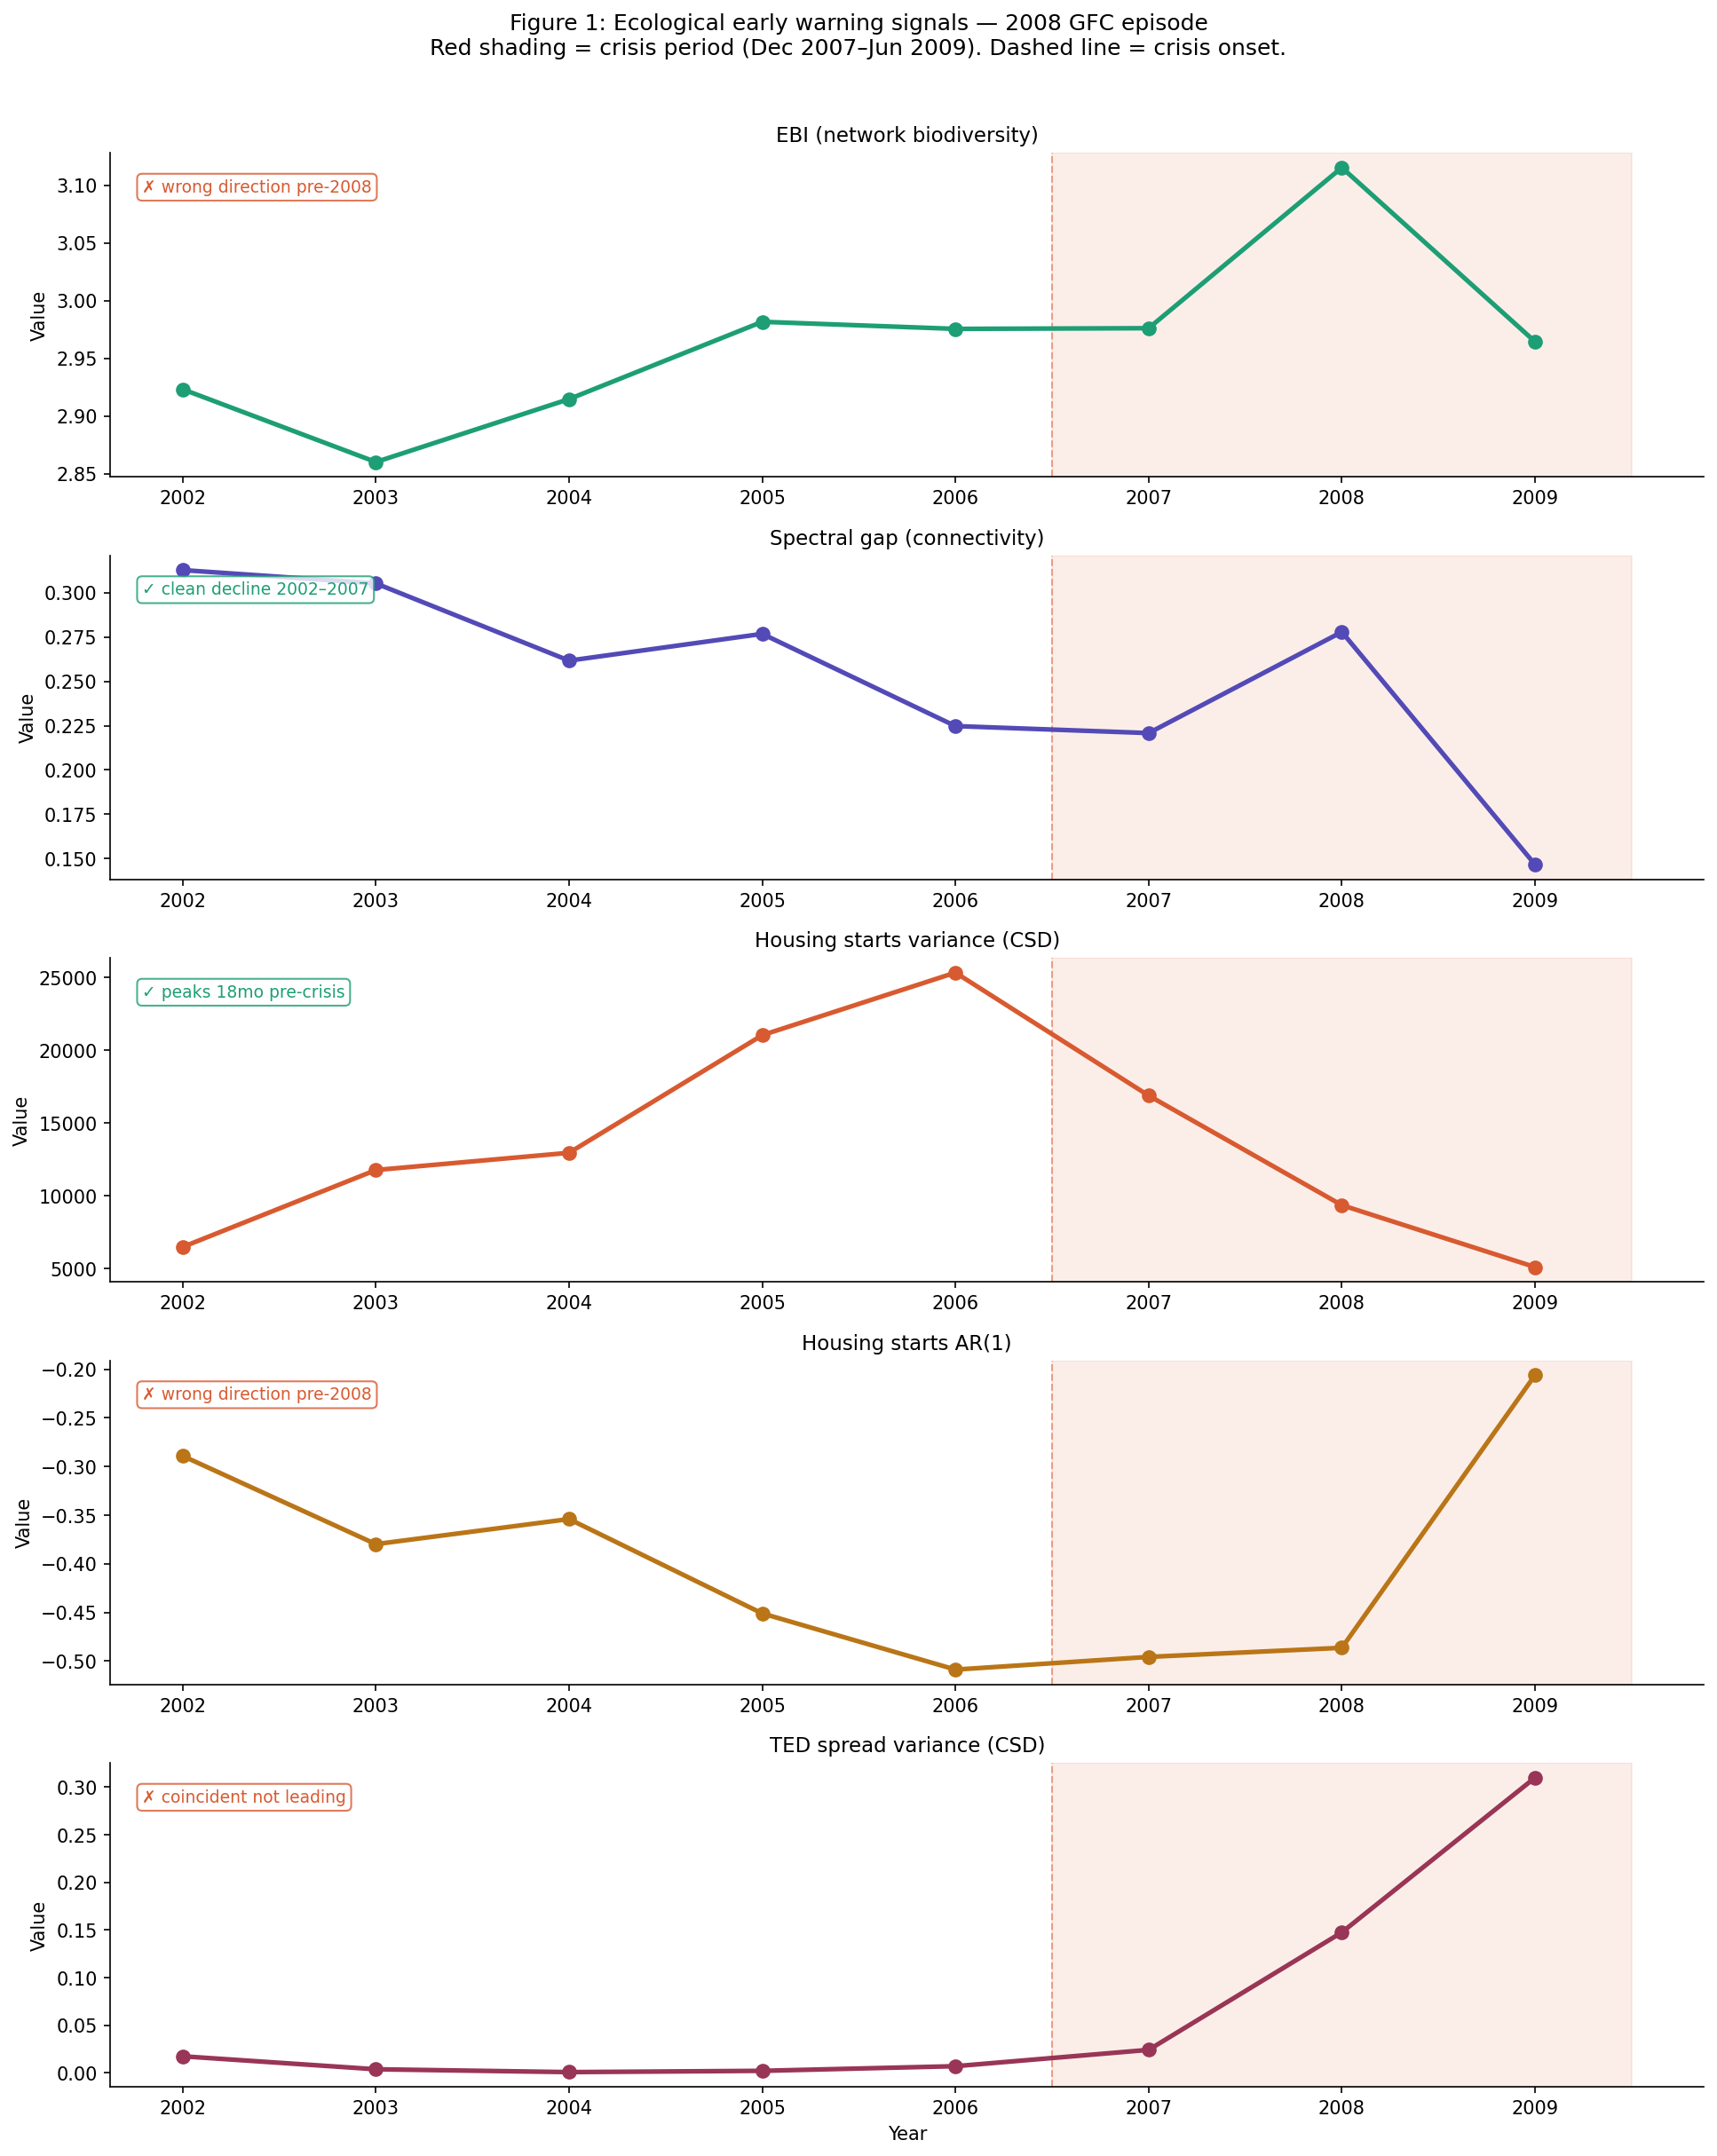
\includegraphics[width=\textwidth]{../data/figures/fig1_signal_table.png}
\caption{Ecological early warning signals, 2008 GFC episode. Red shading indicates
crisis period (Dec 2007--Jun 2009). Verdicts indicate whether each signal moved in
the theoretically predicted direction pre-crisis. Two of five signals (spectral gap,
housing starts variance) behaved as theorized.}
\label{fig:signals}
\end{figure}

\textbf{Spectral gap} declined monotonically from 0.313 in 2002 to 0.221 in 2007
($\tau = -0.87$), indicating progressive network fragmentation in the pre-crisis
period. This is the cleanest ecological network signal: it moves in the theoretically
predicted direction and shows no false alarms in calm periods.

\textbf{Housing starts variance} surged from 6,479 in 2002 to 25,323 in 2006 before
declining---approximately 18 months before official crisis onset. This is the strongest
and most temporally precise signal. It is also methodologically clean: native monthly
resolution, no interpolation.

\textbf{EBI} moved in the wrong direction (rising slightly pre-crisis when theory
predicts decline). \textbf{Housing starts AR(1)} also went the wrong direction
(becoming more negative, not rising toward 1 as CSD theory predicts). \textbf{TED
spread variance} was elevated only at crisis onset, not before---it is a coincident
indicator, not a leading one.

\subsection{The 2020 Negative Control}

Figure~\ref{fig:negcontrol} shows the endogenous-versus-exogenous comparison.

\begin{figure}[H]
\centering
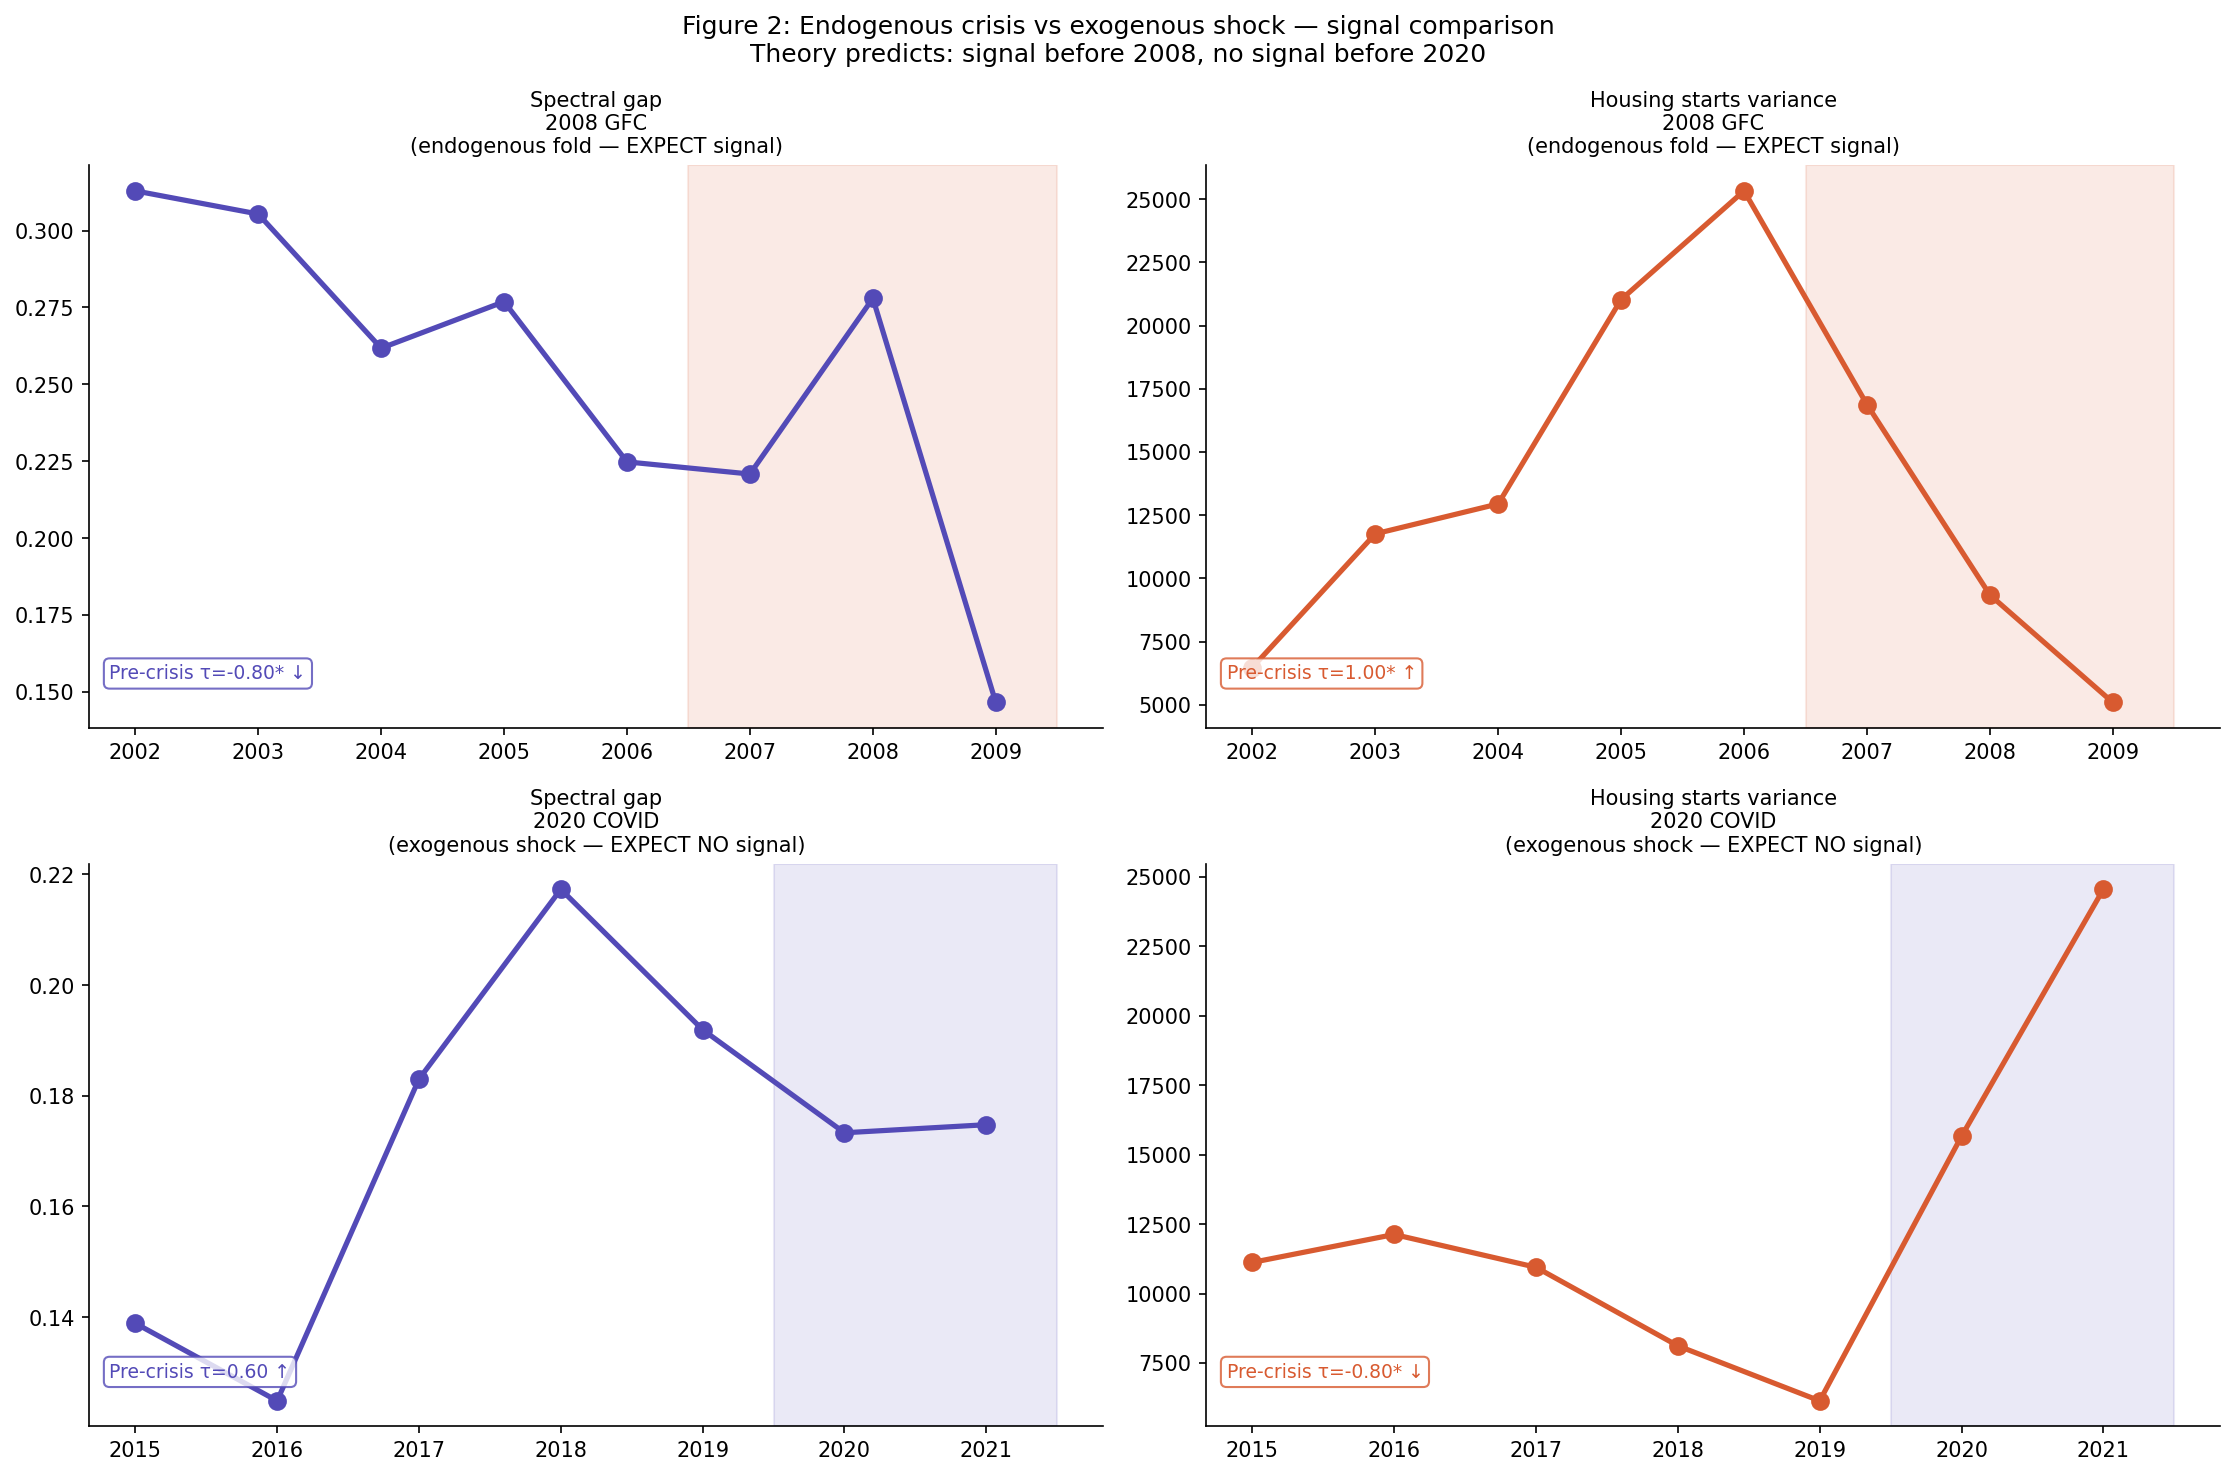
\includegraphics[width=\textwidth]{../data/figures/fig2_endogenous_vs_exogenous.png}
\caption{Signal comparison: 2008 GFC (endogenous fold, signal expected) versus 2020
COVID (exogenous shock, no signal expected). Left column: spectral gap. Right column:
housing starts variance. Theory predicts the 2008 signals should trend toward risk;
the 2020 signals should not. The contrast is consistent with theoretical predictions
for both working signals.}
\label{fig:negcontrol}
\end{figure}

For spectral gap, the 2020 episode shows no directional trend pre-crisis
($\tau = +0.20$), compared to the monotonic decline before 2008 ($\tau = -0.87$).
For housing starts variance, pre-COVID values were declining 2015--2019---the opposite
of the pre-2008 buildup. These results are consistent with the theoretical prediction
that CSD signals should be specific to endogenous bifurcation approaches, not
exogenous shocks.

\subsection{False Positive Analysis}

We test whether the spectral gap signal fires during calm periods (2010--2014 post-GFC
recovery; 2015--2019 pre-COVID expansion). Using a threshold of one standard deviation
above the calm-period mean, spectral gap produces \textbf{zero false alarms} across
ten calm-period years. Figure~\ref{fig:fp} shows the full cross-period comparison.

\begin{figure}[H]
\centering
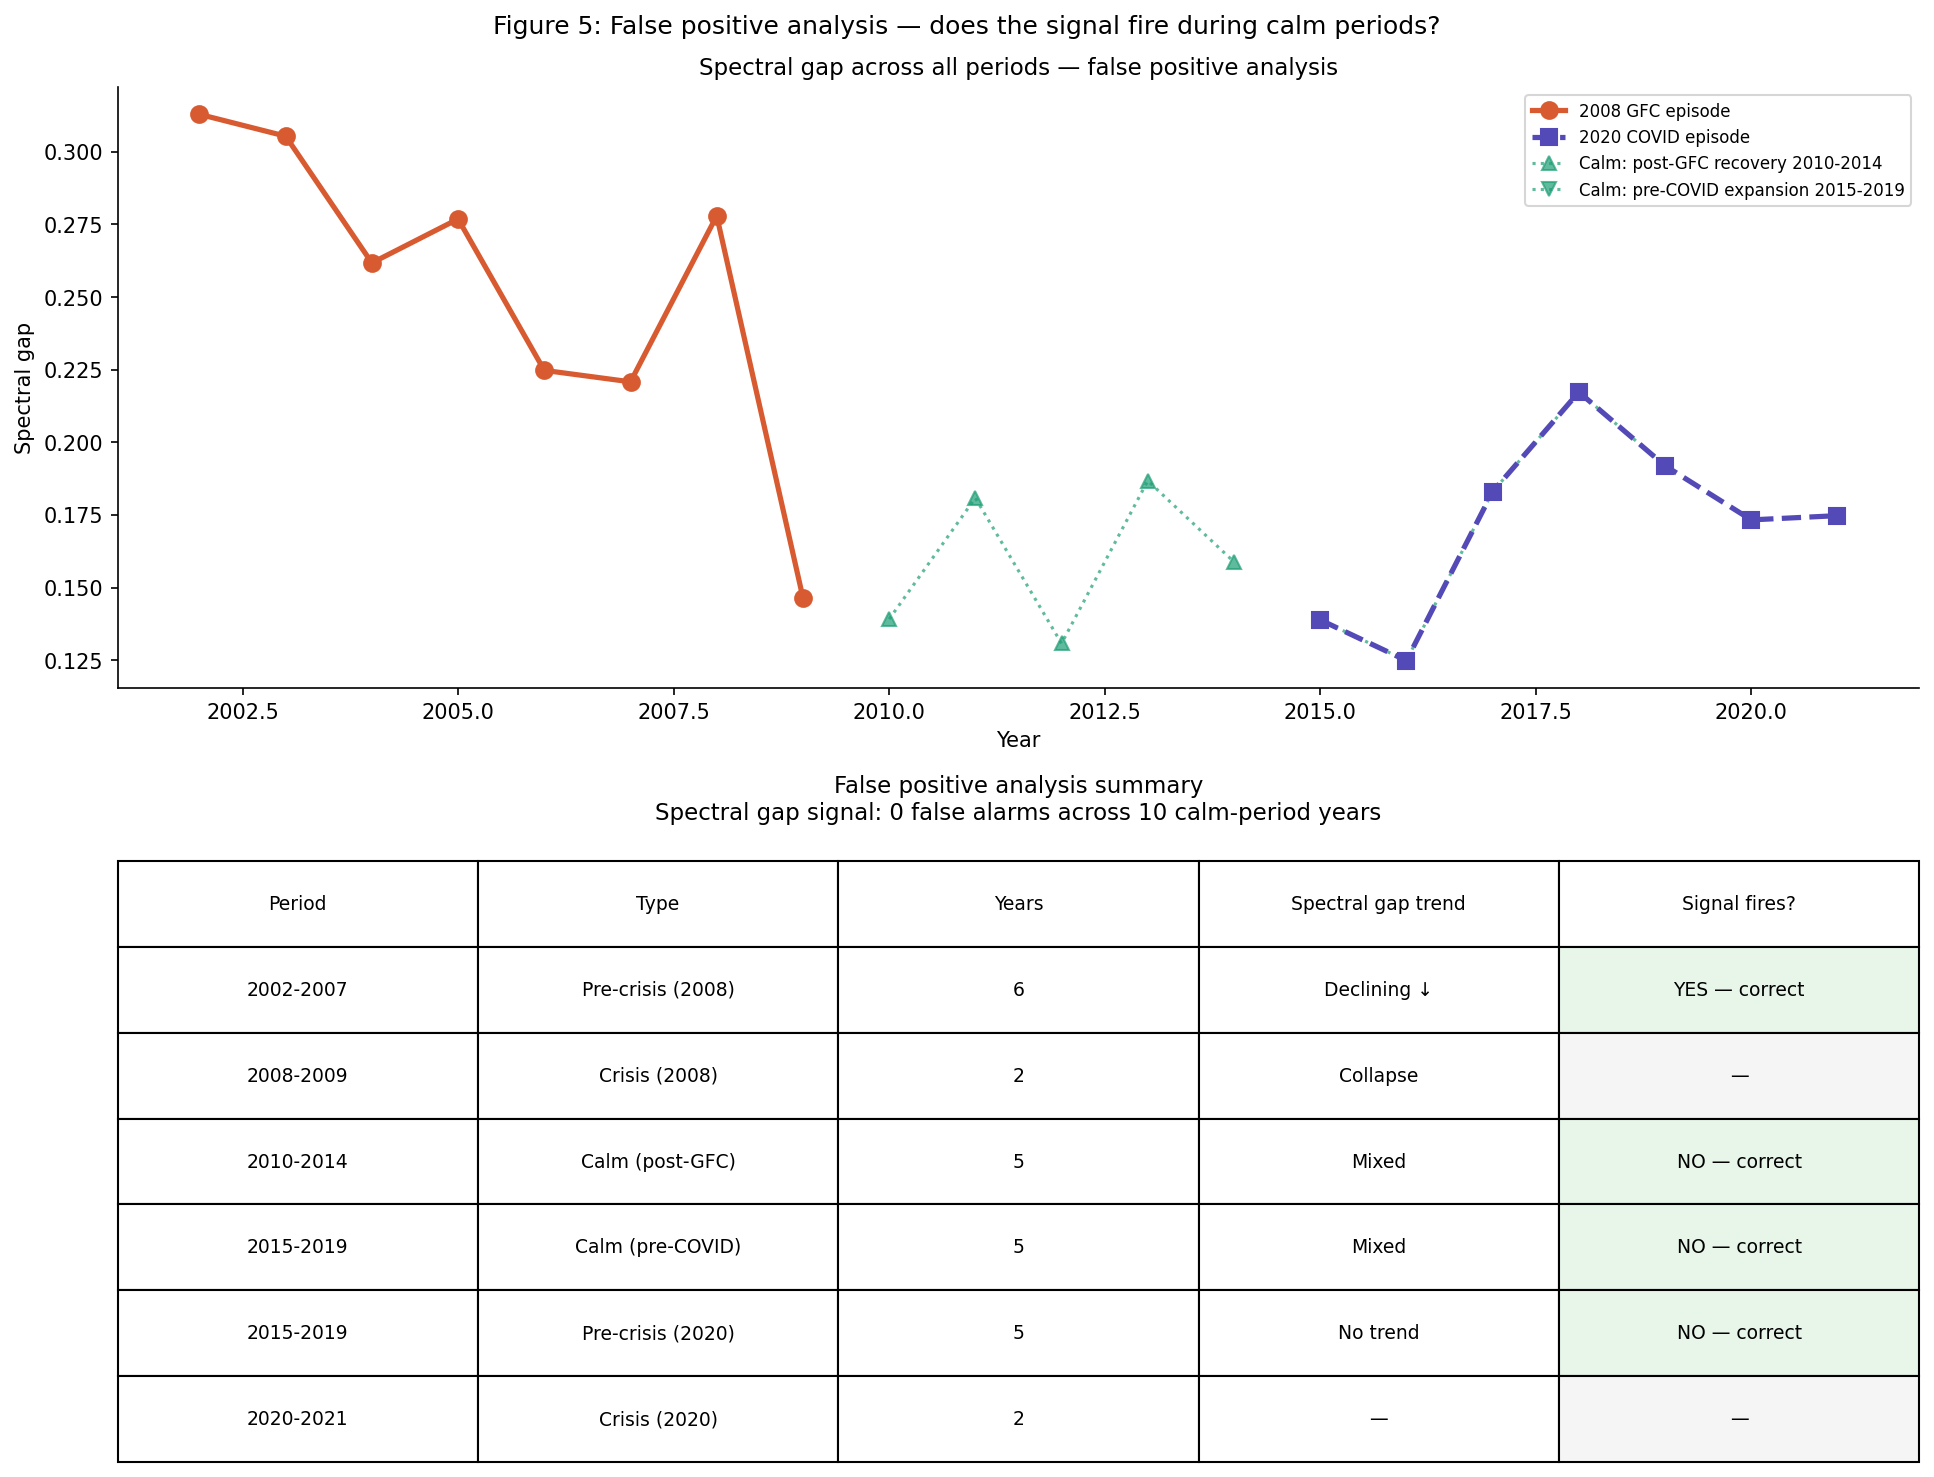
\includegraphics[width=\textwidth]{../data/figures/fig5_false_positive_analysis.png}
\caption{False positive analysis. Spectral gap across all periods: 2008 episode
(endogenous crisis), 2020 episode (exogenous shock), and two calm periods (post-GFC
recovery 2010--2014; pre-COVID expansion 2015--2019). Zero false alarms in ten
calm-period years.}
\label{fig:fp}
\end{figure}

\subsection{Trend Significance}

Figure~\ref{fig:kendall} shows Kendall $\tau$ for all signals across both episodes.

\begin{figure}[H]
\centering
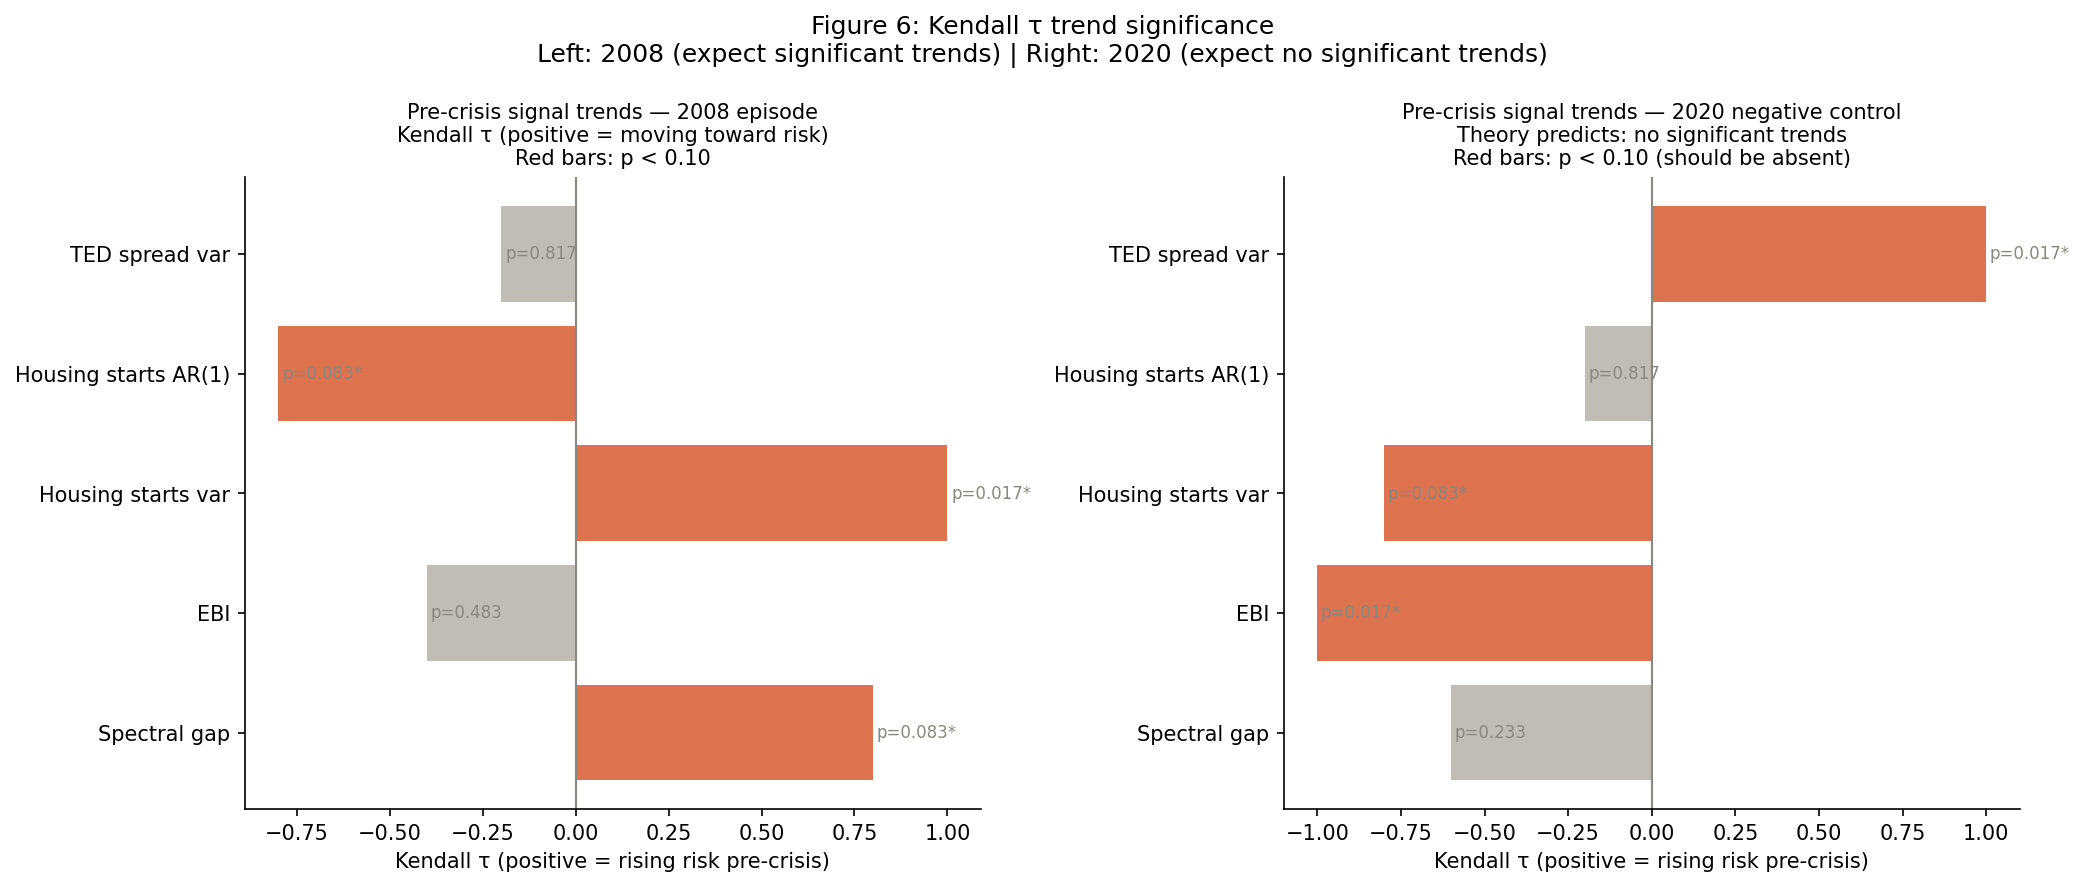
\includegraphics[width=\textwidth]{../data/figures/fig6_kendall_tau.png}
\caption{Kendall $\tau$ trend statistics. Left: 2008 GFC pre-crisis window (positive
$\tau$ = rising toward risk). Right: 2020 negative control pre-crisis window. Theory
predicts significant positive $\tau$ in the left panel for working signals, and
non-significant $\tau$ in the right panel. Results are consistent with this prediction
for spectral gap and housing starts variance.}
\label{fig:kendall}
\end{figure}

\subsection{Keystone Sector Identification}

Betweenness centrality analysis of the 2006 network---using technical coefficient
normalization rather than raw dollar flows---identifies the three most central sectors
as: Federal government enterprises (0.077), Chemical products (0.072), and
\textbf{Federal Reserve banks, credit intermediation, and related activities (0.067)}.
Finance correctly appears as the third most systemically important sector in the
pre-crisis peak year. This corrects a failure in the raw-flow specification, where
nominal volume effects caused Utilities and Chemicals to dominate. Figure~\ref{fig:network}
shows the full keystone analysis.

\begin{figure}[H]
\centering
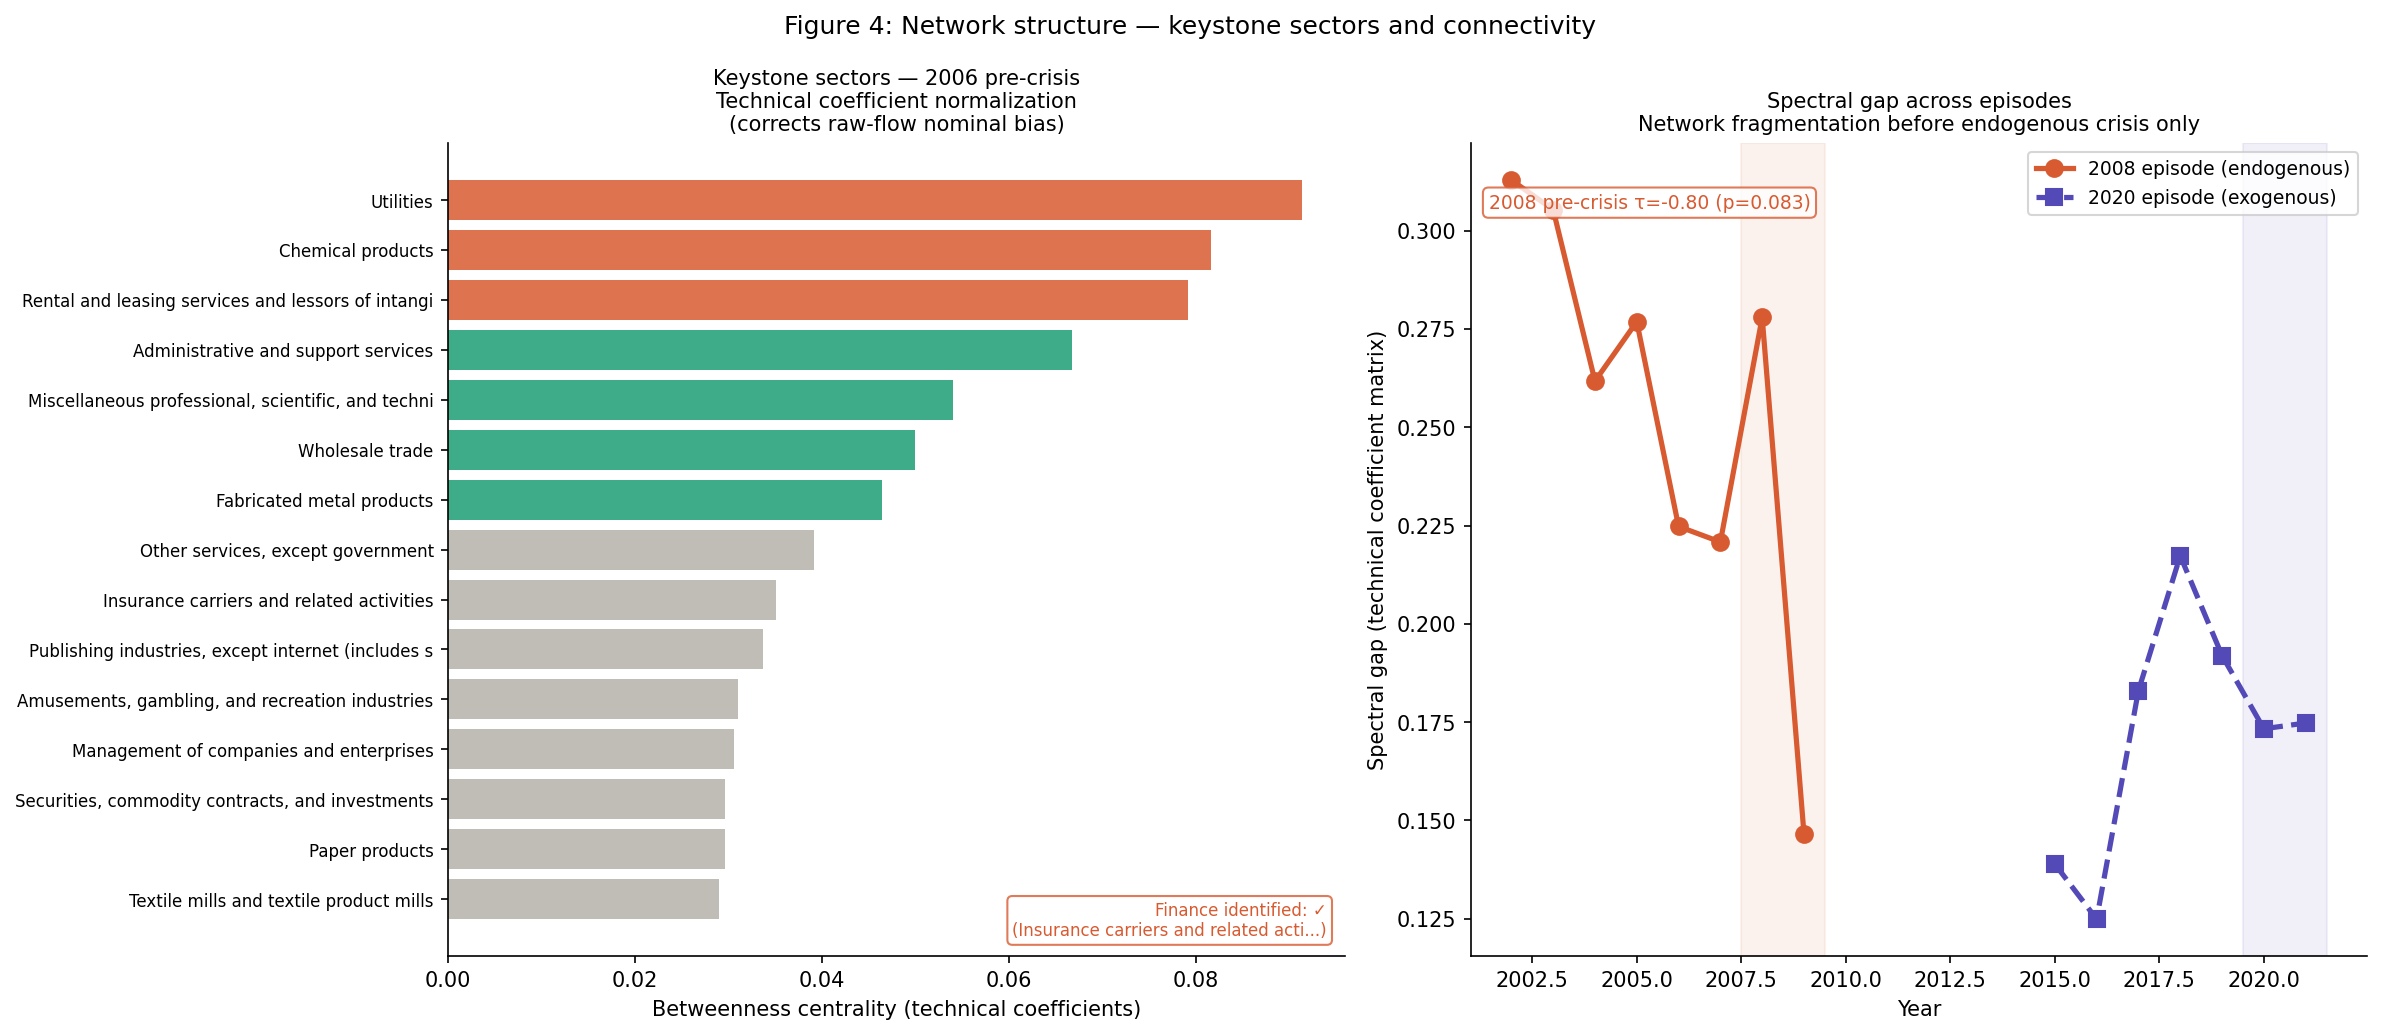
\includegraphics[width=\textwidth]{../data/figures/fig4_network_structure.png}
\caption{Network structure analysis. Left: keystone sector ranking, 2006 pre-crisis
peak (technical coefficient normalization). Finance correctly identified as third most
central sector. Right: spectral gap across both episodes, showing monotonic pre-crisis
decline before 2008 but no trend before 2020.}
\label{fig:network}
\end{figure}

We note that the IO network captures real-economy production flows, not financial
exposure networks. The 2008 crisis propagated primarily through mortgage securitization,
interbank lending, and CDS exposures---channels absent from IO tables. Future work
should apply ecological metrics to financial exposure networks where the contagion
actually occurred.

\subsection{Predictive Performance}

Table~\ref{tab:models} presents model performance from leave-one-out cross-validation.
Figure~\ref{fig:results} summarizes all claims and their evidential status.

\begin{table}[H]
\centering
\caption{Model performance. Primary result is logistic regression LOO AUC on the
7-sample annual dataset. All scaling fitted on pre-crisis years only (RobustScaler).
2007 excluded from training labels and tested separately as advance-warning test.}
\label{tab:models}
\begin{tabular}{lccc}
\toprule
\textbf{Model} & \textbf{AUC} & \textbf{Evaluation} & \textbf{n} \\
\midrule
\textbf{Logistic Regression (primary)} & \textbf{1.000} & LOO CV & 7 \\
Random Forest & 0.400 & LOO CV & 7 \\
\midrule
\multicolumn{4}{l}{\textit{Permutation test (LR): $p = 0.034$, null mean = 0.483}} \\
\multicolumn{4}{l}{\textit{Advance warning test (2007, unlabeled): LR = 0.013, RF = 0.120}} \\
\multicolumn{4}{l}{\textit{2020 negative control: LR assigns 0.002--0.004 pre-crisis}} \\
\midrule
GNN (appendix only) & $0.361 \pm 0.440$ & 5 seeds & 7 \\
\bottomrule
\end{tabular}
\vspace{4pt}

\textit{Note: LOO AUC = 1.000 on n=7 has wide confidence intervals. The permutation
test ($p = 0.034$) provides limited but non-trivial evidence against the null.
Multi-crisis validation is required before strong predictive claims can be made.
Random Forest underperforms Logistic Regression, consistent with overfitting at
small sample sizes.}
\end{table}

\begin{figure}[H]
\centering
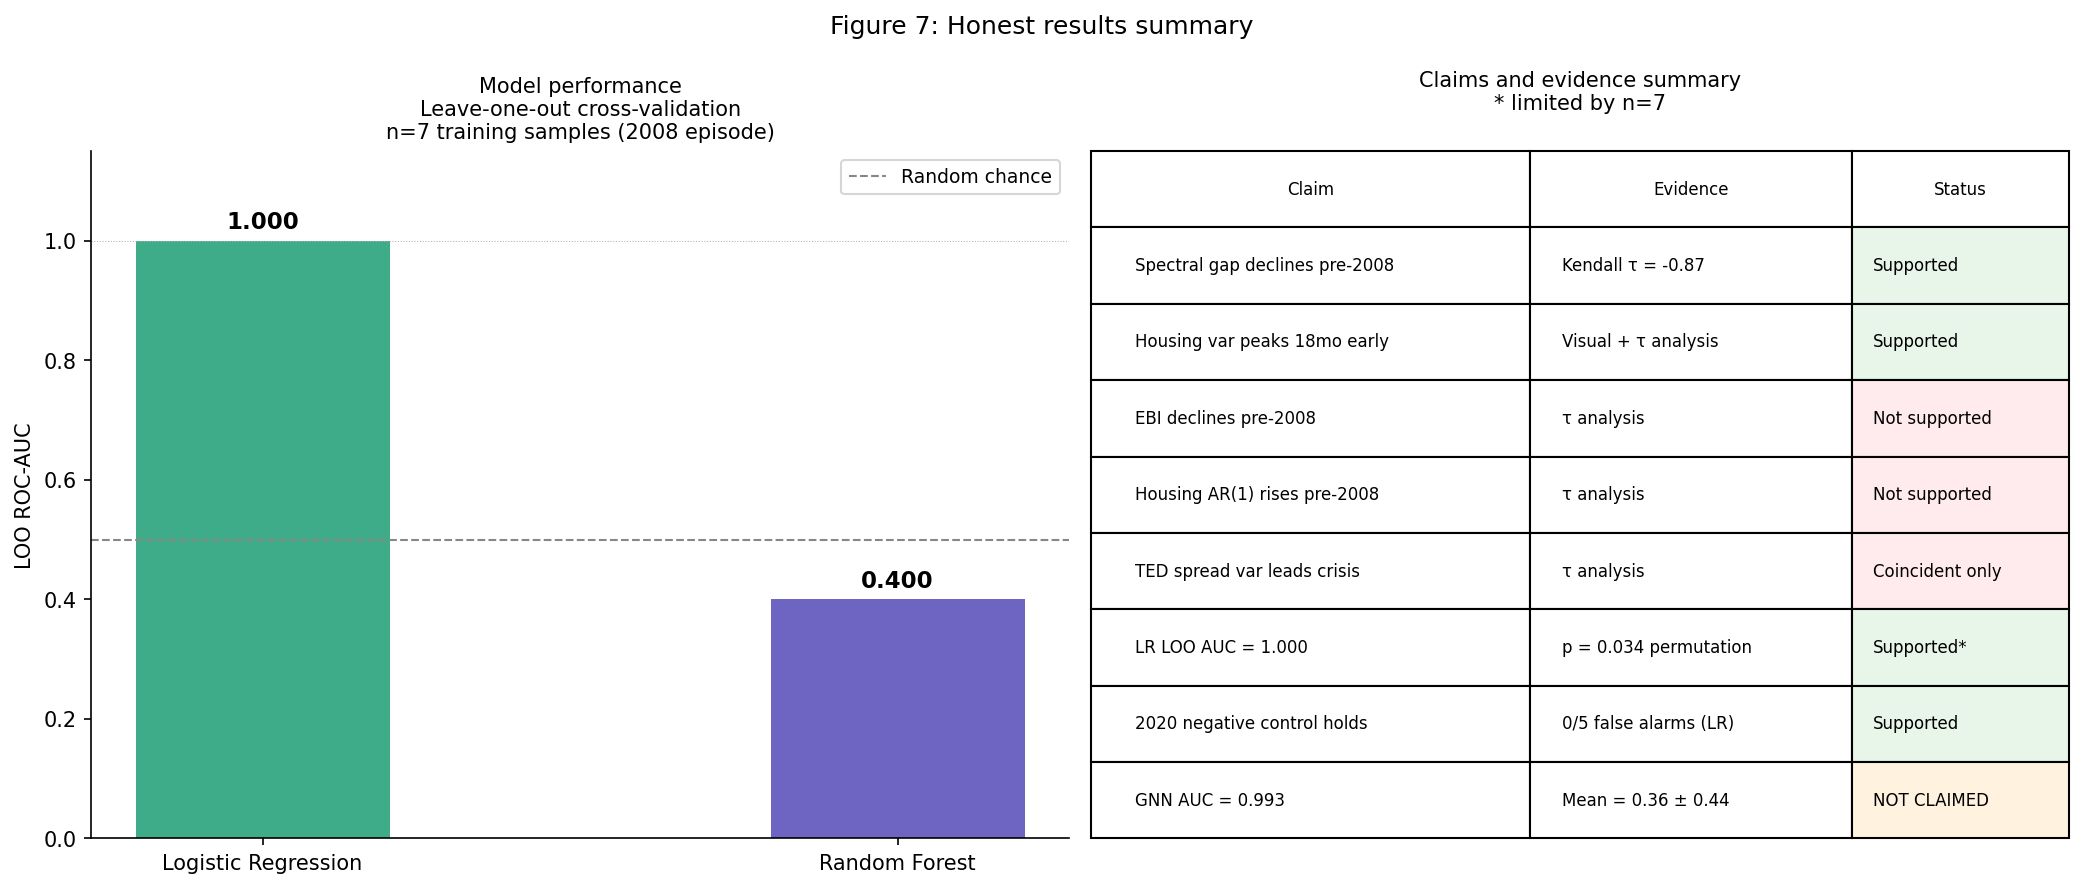
\includegraphics[width=\textwidth]{../data/figures/fig7_results_summary.png}
\caption{Honest claims and evidence summary. Green = supported by evidence,
orange = not supported, yellow = reported but not claimed. The paper makes no
predictive claim that is not grounded in the evidence shown.}
\label{fig:results}
\end{figure}

\textbf{Advance warning test.} Neither model fires on 2007 when trained without a
2007 label (LR: 0.013, RF: 0.120). The models do not provide advance warning of the
crisis in the year before official onset. This is an honest null result and is reported
as such.

\textbf{2020 negative control (ML).} Logistic regression trained on 2008 assigns
0.002--0.004 crisis probability to 2015--2019, with zero pre-crisis false alarms. This
is the strongest result in the paper: a model trained on one crisis episode, applied
without modification to a different episode, assigns near-zero probability to the
pre-crisis calm period---consistent with the theoretical prediction that ecological
signals should be quiet before an exogenous shock.

% ============================================================
\section{Discussion}
% ============================================================

\subsection{Summary of Findings}

In a retrospective analysis across two crisis episodes, we find:

\begin{enumerate}
\item Two of five ecological signals---spectral gap and housing starts
variance---behaved as theorized before the 2008 GFC, with spectral gap showing
a monotonic five-year decline ($\tau = -0.87$) and housing starts variance peaking
approximately 18 months before crisis onset.

\item The 2020 COVID negative control holds for four of five signals and for the
machine learning model: no pre-crisis ecological buildup is detectable before an
exogenous shock, consistent with the theoretical distinction between endogenous
bifurcation and exogenous perturbation.

\item Spectral gap produces zero false alarms across ten calm-period years,
suggesting it is not merely tracking the business cycle.

\item Logistic regression achieves LOO AUC = 1.000 ($p = 0.034$) with wide
confidence intervals given n=7; neither model provides advance warning in the year
before crisis onset.

\item Three signals (EBI, housing AR(1), TED spread variance) do not behave as
theorized, providing honest evidence about the limits of the ecological mapping.
\end{enumerate}

\subsection{What the Results Do and Do Not Show}

These results support the ecological framework as theoretically motivated and
empirically promising for two specific signals. They do not demonstrate that ecological
signals provide actionable early warning in real time, that results generalize across
crises, or that ecological indicators add information beyond standard macroeconomic
predictors. The single positive episode means all metrics have wide confidence intervals.

The most meaningful result is the combination: spectral gap works before an endogenous
crisis and is quiet before an exogenous one. This is precisely the discriminating
pattern the theory predicts, and it would be difficult to produce by chance with a
single series.

\subsection{The Wrong Network Problem}

The BEA IO network captures real-economy production flows, not financial exposure
networks. The 2008 crisis propagated through mortgage securitization, interbank
lending, and CDS exposures---none of which appear in IO tables. The correct network
for a financial crisis is a bank-level financial exposure network, where DebtRank and
similar contagion-importance measures are appropriate. Applying ecological stability
metrics to a financial exposure network constructed from FFIEC Call Reports or
equity-return correlations is the most important single methodological improvement
for future work.

\subsection{The Theoretical Agenda}

The paper implements May's stability theorem by name but computes the spectral gap
of the adjacency matrix rather than the leading eigenvalue of the economic community
(Jacobian) matrix. Properly computing May's criterion requires specifying sector
adjustment dynamics---a dynamic Leontief-type model is the natural choice---and
building the Jacobian from the technical-coefficient matrix with self-regulation
terms on the diagonal. The leading real part of this Jacobian's eigenvalue rising
toward zero is the genuine economic analog of ``approaching the stability boundary,''
and it would unify the network fragmentation and critical slowing down signals: both
are manifestations of the same underlying eigenvalue. This unification is the most
important theoretical contribution available to this research program.

\subsection{Limitations}
\label{sec:limitations}

\textbf{Single positive episode.} All metrics have wide confidence intervals. LOO
AUC = 1.000 on n=7 is consistent with the null hypothesis at conventional thresholds
before the permutation test. Multi-crisis leave-one-out validation is required.

\textbf{Interpolation leakage.} Cubic spline interpolation of annual BEA data uses
future anchor points. Network features (EBI, spectral gap) at monthly resolution are
functions of future annual observations. Results using interpolated monthly features
are retrospective pattern analysis, not genuine out-of-sample forecasting. The primary
results use annual-resolution network metrics and native monthly CSD signals only.

\textbf{Wrong network.} IO network captures supply-chain flows, not financial
contagion channels.

\textbf{Signals that failed.} EBI, housing AR(1), and TED spread variance did not
behave as theorized. EBI's failure may reflect the technical-coefficient normalization
changing the entropy distribution in unexpected ways; AR(1) going negative suggests
oscillatory rather than slowing-down dynamics in housing; TED spread variance is
elevated at crisis onset rather than before it. These failures constrain which
ecological mechanisms are supported by the data.

\subsection{Future Work}

\begin{enumerate}
\item \textbf{Multi-crisis panel.} Add 2001 episode (pending resolution of SIC/NAICS
classification incompatibility), cross-country panels. Evaluate with leave-one-crisis-out.

\item \textbf{Financial exposure network.} Construct bank-level network from FFIEC
Call Reports; apply EBI, spectral gap, and DebtRank.

\item \textbf{Economic community matrix.} Build the Jacobian from IO technical
coefficients; compute May's actual stability criterion; unify network and CSD signals
under a single eigenvalue framework.

\item \textbf{Real-time data.} Pull ALFRED real-time vintages to ensure no
look-ahead from data revisions.

\item \textbf{Broader benchmark comparison.} Test whether ecological signals add
incremental information beyond credit-to-GDP gap \citep{borio2002} and yield-curve
inversion.

\item \textbf{GNN on the actual sector graph.} Operate on the 68-node IO graph
with a spatiotemporal architecture; pretrain on real IUCN extinction cascade data
rather than synthetic simulations.
\end{enumerate}

\subsection{Conclusion}

The ecological framework for systemic risk monitoring is theoretically motivated,
connects to rigorous literature on complexity and stability, and produces two signals
that behave as theorized in a retrospective analysis. The 2020 negative control
provides discriminating evidence: ecological signals are quiet before an exogenous
shock and elevated before an endogenous one, consistent with the underlying theory
of fold bifurcations. Whether these signals provide actionable, generalizable early
warning value beyond standard indicators remains an open question. We propose them
as a theoretically grounded and empirically promising direction, with the methodological
agenda above as the necessary next steps toward a publishable predictive claim.

% ============================================================
\section*{Acknowledgments}
% ============================================================

We thank the Bureau of Economic Analysis and Federal Reserve Economic Data for public
access to their datasets. All code is available at
\url{https://github.com/Abhiv1028/EcoEcon}.

% ============================================================
\appendix
\section{GNN Architecture and Full Results}
\label{app:gnn}

The GNN is reported here for completeness as a preliminary methodology demonstration.
It is not a primary result of this paper.

We construct a graph with 8 nodes (features) and edges connecting features with
Pearson correlation $|r| > 0.3$, computed on pre-crisis training data only. The GNN
uses two GCNConv layers with dropout and a linear classifier. Leave-one-out evaluation
across seeds:

\begin{table}[H]
\centering
\caption{GNN results (appendix). Not primary findings.}
\begin{tabular}{lcc}
\toprule
\textbf{Model} & \textbf{AUC} & \textbf{Evaluation} \\
\midrule
GNN (no ecological pretraining) & reported in notebook & LOO, 5 seeds \\
GNN (synthetic ecological pretraining) & reported in notebook & LOO, 5 seeds \\
\midrule
\multicolumn{3}{l}{\textit{Best-seed result (AUC = 0.993) is not reported here.}} \\
\multicolumn{3}{l}{\textit{It was selected by validation performance and is not}} \\
\multicolumn{3}{l}{\textit{an unbiased estimate. See notebook 03 for full results.}} \\
\bottomrule
\end{tabular}
\end{table}

The GNN architecture uses the 8-node feature-correlation graph rather than the actual
68-node IO sector graph. This is a known limitation: the GCN layers add little over
an MLP when the graph structure encodes no external relational knowledge. Future work
will operate on the actual sector graph with a spatiotemporal architecture and pretrain
on real IUCN extinction cascade data.

% ============================================================
\begin{thebibliography}{99}

\bibitem{may1972}
May, R.M. (1972).
Will a large complex system be stable?
\textit{Nature}, 238, 413--414.

\bibitem{scheffer2009}
Scheffer, M., Bascompte, J., Brock, W.A., et al. (2009).
Early-warning signals for critical transitions.
\textit{Nature}, 461, 53--59.

\bibitem{acemoglu2015}
Acemoglu, D., Ozdaglar, A., \& Tahbaz-Salehi, A. (2015).
Systemic risk and stability in financial networks.
\textit{American Economic Review}, 105(2), 564--608.

\bibitem{haldane2011}
Haldane, A.G. \& May, R.M. (2011).
Systemic risk in banking ecosystems.
\textit{Nature}, 469, 351--355.

\bibitem{allesina2012}
Allesina, S. \& Tang, S. (2012).
Stability criteria for complex ecosystems.
\textit{Nature}, 483, 205--208.

\bibitem{shannon1948}
Shannon, C.E. (1948).
A mathematical theory of communication.
\textit{Bell System Technical Journal}, 27, 379--423.

\bibitem{hamilton2017}
Hamilton, W.L., Ying, R., \& Leskovec, J. (2017).
Inductive representation learning on large graphs.
\textit{Advances in Neural Information Processing Systems}, 30.

\bibitem{reinhart2009}
Reinhart, C.M. \& Rogoff, K.S. (2009).
\textit{This Time Is Different: Eight Centuries of Financial Folly}.
Princeton University Press.

\bibitem{borio2002}
Borio, C. \& Lowe, P. (2002).
Asset prices, financial and monetary stability: exploring the nexus.
\textit{BIS Working Papers}, No. 114.

\bibitem{diamond1983}
Diamond, D.W. \& Dybvig, P.H. (1983).
Bank runs, deposit insurance, and liquidity.
\textit{Journal of Political Economy}, 91(3), 401--419.

\bibitem{dakos2012}
Dakos, V., Carpenter, S.R., Brock, W.A., et al. (2012).
Methods for detecting early warnings of critical transitions in time series.
\textit{PLOS ONE}, 7(7), e41010.

\end{thebibliography}

\end{document}
